\appendix
\xchapter{Ferramentas de teste para apps Android}{}\label{sec:toolsandroid}


\begin{table*}[h!]
\begin{center}
    \scriptsize
    \caption{Ferramentas de teste para apps Android}
    \label{table:androidtools}
    \def \arraystretch{1.2}
    
    \begin{tabular}{m{4cm}m{5cm}m{3cm}m{3cm}}
        \toprule
        \bf Ferramenta & \bf Tipo de Teste & \bf Literatura/Mercado & \bf Gratuita/Proprietária\\ 
        \midrule
        APPIUM \footnote{\url{http://appium.io/}} & Funcional/GUI & Mercado & Gratuita & \\\hline
        ATOM \cite{7927972} & Teste de Regressão & Literatura & Gratuita\\\hline
        CALABASH\footnote{\url{https://github.com/calabash/calabash-android}} & Funcional/GUI & Mercado & Gratuita\\\hline
        CHATEM \cite{8424973} & Teste de Regressão & Literature & Gratuita\\\hline
        DETREDUCE \cite{Choi:2018:DMA:3180155.3180173} & Teste de Regressão & Literature & Gratuita\\\hline
        ESPRESSO\footnote{\url{https://developer.android.com/training/testing/espresso.}} & Funcional/GUI & Mercado & Gratuita\\\hline
        GUIDIFF \cite{6569773} & Teste de Regressão & Literature & Gratuita\\\hline
        KATALON\footnote{\url{https://www.katalon.com/katalon-studio/}} & Funcional/GUI & Mercado & Gratuita\\\hline
        KMAX\footnote{\url{https://iwl.com/products/kmax}} & Performance & Mercado & Proprietária\\\hline
        KOBITON\footnote{\url{https://kobiton.com/}} & Funcional/GUI/Performance & Mercado & Proprietária\\\hline
        MONKEY\footnote{\url{https://developer.android.com/studio/test/monkey}} & Stress & Mercado & Gratuita\\\hline
        MONKEY RUNNER\footnote{\url{https://developer.android.com/studio/test/monkeyrunner}} & Funcional/GUI/Teste de Regressão & Mercado & Gratuita\\\hline
        RANOREX\footnote{\url{https://www.ranorex.com/}} & Funcional/GUI/Teste de Regressão & Mercado & Proprietária\\\hline
        REDROID \cite{Do2016RedroidAR} & Teste de Regressão & Literature & Gratuita\\\hline
        RETESTDROID \cite{8377661} & Teste de Regressão & Literature & Gratuita\\\hline
        ROBOLECTRIC\footnote{\url{http://robolectric.org/}} & Estrutural/Unidade & Mercado & Gratuita\\\hline
        ROBOTIUM\footnote{\url{https://github.com/RobotiumTech/robotium}} & Funcional/GUI & Mercado & Gratuita\\\hline
        SEE TEST\footnote{\url{https://experitest.com/mobile-test-automation}} & Funcional/GUI/Performance & Mercado & Proprietária\\\hline
        SQUISH\footnote{\url{https://www.froglogic.com/squish/editions/automated-android-gui-testing/}} & Funcional/GUI/Teste de Regressão & Mercado & Proprietária\\\hline
        TELERIK\footnote{\url{https://www.telerik.com/teststudio}} & Funcional/GUI & Mercado & Proprietária\\\hline
        TEMA \cite{5770627} & Teste de Regressão & Literature & Gratuita\\\hline
        TESTCOMPLETE\footnote{\url{https://smartbear.com/product/testcomplete/overview/}} & Funcional/GUI/Teste de Regressão & Mercado & Proprietária\\\hline
        TESTINGBOT\footnote{\url{https://testingbot.com/}} & Funcional/GUI/Performance & Mercado & Proprietária\\\hline
        UFT\footnote{\url{https://www.microfocus.com/pt-br/products/uft-one/overview}} & Funcional/GUI/Performance/Teste de Regressão & Mercado & Proprietária\\\hline
        UI AUTOMATOR\footnote{\url{https://developer.android.com/training/testing/ui-automator}} & Funcional/GUI & Mercado & Gratuita\\\hline
\end{tabular}
\end{center}
\end{table*}


\vspace{0.5cm}
% \hline
\footnotesize
{
\textsuperscript{1}\url{http://appium.io/}

\textsuperscript{2}\url{https://github.com/calabash/calabash-android}

\textsuperscript{3}\url{https://developer.android.com/training/testing/espresso}

\textsuperscript{4}\url{https://www.katalon.com/katalon-studio/}

\textsuperscript{5}\url{https://iwl.com/products/kmax}

\textsuperscript{6}\url{https://kobiton.com/}

\textsuperscript{7}\url{https://developer.android.com/studio/test/monkey}

\textsuperscript{8}\url{https://developer.android.com/studio/test/monkeyrunner}

\textsuperscript{9}\url{https://www.ranorex.com/}

\textsuperscript{10}\url{http://robolectric.org/}

\textsuperscript{11}\url{https://github.com/RobotiumTech/robotium}

\textsuperscript{12}\url{https://experitest.com/mobile-test-automation}

\textsuperscript{13}\url{https://www.froglogic.com/squish/editions/automated-android}

\textsuperscript{14}\url{https://www.telerik.com/teststudio}

\textsuperscript{15}\url{https://smartbear.com/product/testcomplete/overview/}

\textsuperscript{16}\url{https://testingbot.com/}

\textsuperscript{17}\url{https://www.microfocus.com/pt-br/products/uft-one/overview}

\textsuperscript{18}\url{https://developer.android.com/training/testing/ui-automator}
}





\xchapter{Questionário \textit{survey}}{}\label{sec:formulariopesquisa}


Prezado colaborador, este questionário destina-se a coletar dados para um trabalho acadêmico de mestrado em Ciência da Computação da Universidade Federal da Bahia (UFBA), com objetivo de investigar a aplicação de teste de regressão no desenvolvimento de \ac{APPS} Android. A sua participação é de fundamental importância.


\begin{enumerate}[label=\bf A\arabic*,leftmargin=1.8cm]

    \item \textbf{TERMO DE CONSENTIMENTO LIVRE E ESCLARECIDO}
    


    \begin{enumerate}[label= \arabic*]
    
        \item O/A senhor(a) está sendo convidada(o) a participar voluntariamente da pesquisa sobre processo de teste de \ac{APPS} Android.

        \iten Sua participação não é obrigatória.

        \item A qualquer momento você pode desistir de participar e retirar seu consentimento.

        \item Sua recusa não trará nenhum prejuízo em sua relação com a pesquisadora ou com a instituição.

        \item Este formulário tem por objetivo investigar o processo de teste de \ac{APPS} Android.

        \item Sua participação neste formulário consistirá em responder questões objetivas e subjetivas.
 
        \item Sua identificação é opcional, ou seja, você não precisa informar nome ou e-mail caso assim deseje.

        \item A aplicação do formulário está sendo realizada por Sara Mendes Oliveira Lima, estudante da pós graduação em Ciência da Computação na Universidade Federal da Bahia, sob a supervisão do Prof. Dr. Ivan C. Machado.

        \item Os benefícios relacionados à sua participação estão apenas em contribuir com a pesquisa científica. Será permitido acesso aos resultados desta pesquisa por meio da dissertação ou publicações científicas realizadas a partir desse estudo.

        \item As informações pessoais obtidas através desta pesquisa serão confidenciais e não serão distribuídas ou divulgadas pela pesquisadora.

        \item Os dados coletados neste formulário não serão divulgados de forma a possibilitar sua identificação.

        \item Ao continuar respondendo este questionário, o/a senhor(a) concorda com as informações aqui descritas, porém a qualquer momento o/a senhor(a) poderá interromper a pesquisa sem ônus algum.

        \item Este questionário utiliza o pacote de aplicativo Google Docs, portanto a coleta e o uso de informações do Google estão sujeitos à Política de privacidade do Google (https://www.google.co.uk/policies/privacy/).

        \item Abaixo seguem os dados de contato dos responsáveis por esta pesquisa, com os quais você pode tirar suas dúvidas sobre sua participação.\\
        
        Pesquisadores responsáveis:
        
        
        Sara Mendes Oliveira Lima - lima.sara@ufba.br
        
        Ivan C. Machado, Ph.D. - ivan.machado@ufba.br (supervisor). 
        
        Universidade Federal da Bahia (UFBA)
        
        Instituto de Matemática e Estatística
        
        Departamento de Ciência da Computação
        
        Av. Adhemar de Barros, s/n, sala 280, Ondina, 40170-110, Salvador – BA\\
   
        
        Salvador - Ba, Janeiro de 2020.

    \end{enumerate}
    
    
    
    \textbf{Declaro que entendi os objetivos, riscos e benefícios de minha participação na pesquisa.*}

    \begin{itemize}
        \item \textbf{Concordo}
    \end{itemize}
    
    

    \item \textbf{PERFIL DO PARTICIPANTE}
    
    Essa sessão tem como objetivo identificar o perfil do respondente, tipo de trabalho realizado e aptidões técnicas.
    
     \begin{enumerate}[label= \arabic*]
     
        \item \textbf{Gênero: *}\\
        (múltipla escolha)
        \begin{itemize}
            \item Homem
            \item Mulher
            \item Outros
        \end{itemize}
        
        \item \textbf{Idade: *}\\
        (questão subjetiva)
        
        \item \textbf{Nível de Escolaridade: *}\\
        (múltipla escolha)
        \begin{itemize}
            \item Nível médio completo
            \item Curso Técnico completo
            \item Graduação completa
            \item Especialização completa
            \item Mestrado completo
            \item Doutorado completo
            \item Pós-Doutorado
            \item Outros
        \end{itemize}
        
        \item \textbf{Área de Formação Acadêmica: *}\\
        (múltipla escolha)
        \begin{itemize}
            \item Informática, Computação ou áreas afins
            \item Engenharia Elétrica
            \item Engenharia de Produção
            \item Outras Engenharias
            \item Outros
        \end{itemize}
        
        \item \textbf{Você já fez algum curso / certificação na área de testes? *}\\
        (múltipla escolha)
        \begin{itemize}
            \item Sim
            \item Não
        \end{itemize}
        
        \item \textbf{Caso a pergunta acima tenha sido "Sim", quais foram esses cursos / certificações?}\\
        (questão subjetiva)
        
        \item \textbf{Em relação a projetos de \ac{APPS} Android, você: *}\\
        (caixa de seleção)
        \begin{itemize}
            \item Trabalha de forma autônoma
            \item Trabalha / pesquisa em uma empresa
            \item Estudante da área
            \item Outros
        \end{itemize}

        \item \textbf{Estado onde trabalha / estuda: *}\\
        (múltipla escolha)
        \begin{itemize}
            \item Acre
            \item Alagoas
            \item Amapá
            \item Amazonas
            \item Bahia
            \item Ceará
            \item Distrito Federal
            \item Espírito Santo
            \item Goiás
            \item Maranhão
            \item Mato Grosso
            \item Mato Grosso do Sul
            \item Minas Gerais
            \item Pará
            \item Paraíba
            \item Paraná
            \item Pernambuco
            \item Piauí
            \item Rio de Janeiro
            \item Rio Grande do Norte
            \item Rio Grande do Sul
            \item Rondônia
            \item Roraima
            \item Santa Catarina
            \item São Paulo
            \item Sergipe
            \item Tocantins
            \item Outros
        \end{itemize}
        
        
        \item \textbf{Experiência profissional na área de TESTES DE SOFTWARE: *}\\
        (múltipla escolha)
        \begin{itemize}
            \item Até 1 ano
            \item De 1 a 3 anos
            \item De 3 a 5 anos
            \item De 5 a 10 anos
            \item Acima de 10 anos
        \end{itemize}
        
        \item \textbf{Experiência profissional na área específica de TESTES DE APPS ANDROID: *}\\
        (múltipla escolha)
        \begin{itemize}
            \item Até 1 ano
            \item De 1 a 3 anos
            \item De 3 a 5 anos
            \item De 5 a 10 anos
            \item Acima de 10 anos
        \end{itemize}
        
        \item \textbf{Quando comparado a outros profissionais, como você considera o seu nível de conhecimento em TESTES DE \ac{APPS} ANDROID? *}\\
        (múltipla escolha)
        \begin{itemize}
            \item Muito baixo
            \item Baixo
            \item Regular
            \item Bom
            \item Excelente
        \end{itemize}
        
        \item \textbf{Caso seja funcionário de uma empresa, qual a sua principal função no projeto atual?}\\
        (questão subjetiva)
        
        \item \textbf{Qual(is) atividade(s) realiza no processo de teste de software: *}\\
        (caixa de seleção)
        \begin{itemize}
            \item Trabalha com criação / design de casos de teste
            \item Trabalha com execução de casos de teste
            \item Outro
        \end{itemize}        
        
     \end{enumerate}
     
     
    
     \item \textbf{PROCESSO DE TESTES DE \AC{APPS} ANDROID:}
     
     
     As perguntas a seguir referem-se ao processo de teste de \ac{APPS} Android que você realiza. Utilize como base o comportamento encontrado no seu dia-a-dia de trabalho.
     
     \begin{enumerate}[label= \arabic*]
     
     \item \textbf{Os testes realizados se enquadram em qual(is) categorias: *}\\
    (caixa de seleção)
     \begin{itemize}
         \item Funcionais, também conhecido como black-box, quando não há acesso ao código fonte.
         \item Não-funcionais, também conhecido como white-box, quando há acesso ao código fonte.
         \item Grey-box, quando há acesso parcial ao código fonte.
         \item Outros
     \end{itemize}
     
    \item \textbf{Qual(is) tipos de testes a empresa realiza durante o processo de desenvolvimento \ac{APPS} Android?}\\
    (caixa de seleção)
    \begin{itemize}
        \item Teste de GUI
        \item Teste de Unidade
        \item Teste de Integração
        \item Teste de Validação
        \item Teste de Sistema
        \item Teste de Recuperação
        \item Teste de Proteção
        \item Teste de Estresse
        \item Teste de Desempenho
        \item Teste de Conectividade
        \item Teste de Segurança
        \item Teste em Condições Naturais
        \item Teste de Certificação
        \item Teste de Regressão
        \item Outros
    \end{itemize}
     
    \item \textbf{Os testes são realizados de forma: *}\\
    (múltipla escolha)
     \begin{itemize}
        \item Manual
        \item Automatizada
        \item Ambas as formas
     \end{itemize}
    
     \item \textbf{Quais ferramentas você costuma utilizar em seus projetos de \ac{APPS} ANDROID? *}\\
     (caixa de seleção)
     \begin{itemize}
         \item APPIUM
         \item CALABASH
         \item ESPRESSO
         \item KATALON
         \item KMAX
         \item KOBITON
         \item MONKEY
         \item ROBOELETRIC
         \item ROBOTIUM
         \item SEE TEST
         \item TELERIK
         \item TESTINGBOT
         \item UI AUTOMATOR
         \item Não utilizo ferramentas
         \item Outros
     \end{itemize}
     
    \item \textbf{Quando é realizada uma MANUTENÇÃO (ATUALIZAÇÃO) no app Android, quer seja perfectiva, corretiva, adaptativa ou preventiva, é realizado algum tipo de teste com o objetivo de garantir que as manutenções realizadas não alteraram o comportamento funcional do app? *}\\
    (múltipla escolha)
    \begin{itemize}
        \item Nunca
        \item Raramente
        \item Às vezes
        \item Muitas vezes
        \item Sempre
    \end{itemize}
    
    \item \textbf{Caso, a resposta anterior seja positiva, o processo de teste durante a MANUTENÇÃO (ATUALIZAÇÃO) do app é feita de que forma? *}\\
    (múltipla escolha)
    \begin{itemize}
        \item Manual, sem uso de ferramentas
        \item Automatizada, com uso de ferramentas
        \item Ambas
        \item Não testo o aplicativo após MANUTENÇÃO (ATUALIZAÇÃO)
    \end{itemize}
    
    \item \textbf{Quais processos você realiza para testar a versão atualizada do app: *}\\
    (caixa de seleção)
    \begin{itemize}
        \item Reexecuta todos os casos de teste da versão original para testar a versão atualizada do app
        \item Seleciona os casos de teste referente as mudanças entre a versão original e a versão atualizada do app
        \item Avalia se há a necessidade de criar novos casos de teste para a versão atualizada do app
        \item Exclui casos de teste que não são relevadores de falhas para a versão atualizada do app
        \item Reutiliza alguns casos de teste da versão original do app
        \item Não testo o aplicativo após MANUTENÇÃO (ATUALIZAÇÃO)
        \item Outros
    \end{itemize}
    
    \item \textbf{Quando realiza alguma MANUTENÇÃO (ATUALIZAÇÃO) utiliza alguma ferramenta para automatizar o teste da nova versão do APP ANDROID? *}\\
    (múltipla escolha)
    \begin{itemize}
        \item Sim
        \item Não
    \end{itemize}
    
    \item \textbf{Caso utilize, qual(is) são a(s) ferramenta(s)? *}\\
    (caixa de seleção)
    \begin{itemize}
        \item ATOM
        \item CHATEM
        \item DETREDUCE
        \item GUIDIFF
        \item MONKEYRUNNER
        \item RANOREX
        \item REDROID
        \item RETESTDROID
        \item SQUISH
        \item TEMA
        \item TESTCOMPLETE
        \item UFT
        \item Não utilizo ferramentas
        \item Não testo o aplicativo após MANUTENÇÃO (ATUALIZAÇÃO)
        \item Outros
    \end{itemize}
    
    \item \textbf{A(s) ferramenta(s) utilizada(s) atendem as necessidades para testar o app após ATUALIZAÇÃO (MANUTENÇÃO)? *}\\
    (múltipla escolha)
    
    \begin{itemize}
        \item Nunca
        \item Raramente
        \item Às vezes
        \item Muitas vezes
        \item Sempre
        \item Não testo o aplicativo após MANUTENÇÃO (ATUALIZAÇÃO)
    \end{itemize}
    
    \item \textbf{Justifique a resposta anterior: *}\\
    (questão subjetiva)
    
    \item \textbf{Considera relevante testar apps ao realizar algum tipo de MANUTENÇÃO (ATUALIZAÇÃO)? *}\\
    (múltipla escolha)
    \begin{itemize}
        \item Sim
        \item Não
    \end{itemize}
    
    \item \textbf{Qual(is) fator(es) você considera que fazem com que não sejam feitos testes em aplicativos após realização de MANUTENÇÃO (ATUALIZAÇÃO): *}\\
    (caixa de seleção)
    \begin{itemize}
        \item Alto esforço da equipe de teste
        \item Baixa importância na revelação de erros da nova versão
        \item Falta de ferramentas eficientes para automatização desse processo
        \item Tempo Reduzido para entrega da versão atualizada
        \item Outros
    \end{itemize}
    
    \item \textbf{Na sua opinião, quais são as features / funcionalidades que as ferramentas de teste precisam implementar para melhorar / automatizar o processo de testes  durante a manutenção de apps Android? Justifique sua resposta. *}
    (questão subjetiva)
    
    \item \textbf{Você está satisfeito(a) com as features  / funcionalidades oferecidas pelas ferramentas de testes de app Android existentes? *}\\
    (múltipla escolha)
    \begin{itemize}
        \item Sim
        \item Não
    \end{itemize}
    
    \item \textbf{Justifique a sua resposta. *}\\
    (questão subjetiva)
    
    \end{enumerate}
    
    \item \textbf{CONSIDERAÇÕES FINAIS:}
    
    Agradecemos sua participação nessa pesquisa acadêmica. Ela é de fundamental importância para o estudo da área de testes de apps Android.\\
    
    
    Caso queira receber os resultados desse survey, fineza informar o seu e-mail:
    (questão subjetiva)
    
\end{enumerate}



\xchapter{Tabulação de Resultados}{}\label{sec:resultadospesquisa}


Essa seção tem como objetivo apresentar a tabulação de resultados do \textit{survey} realizado.

%\begin{itemize}


    %\item Figura \ref{figure:s_genero}: Gênero.
        \begin{figure}[!htb]
        \centering
        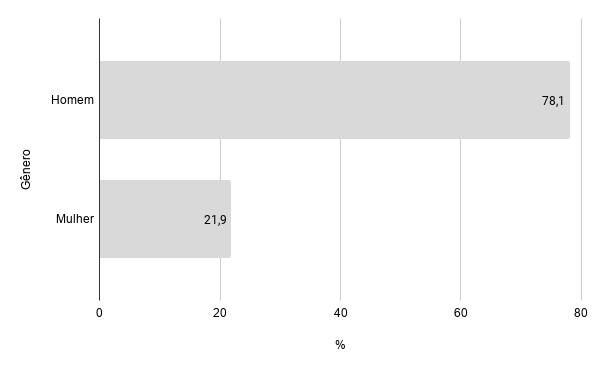
\includegraphics[width=.70\textwidth]{images/s_genero.png}
        \label{figure:s_genero}
        \caption{Gênero.}
        \end{figure}
    
    
    %\item Figura \ref{figure:s_idade}: Idade.
        \begin{figure}[!htb]
        \centering
        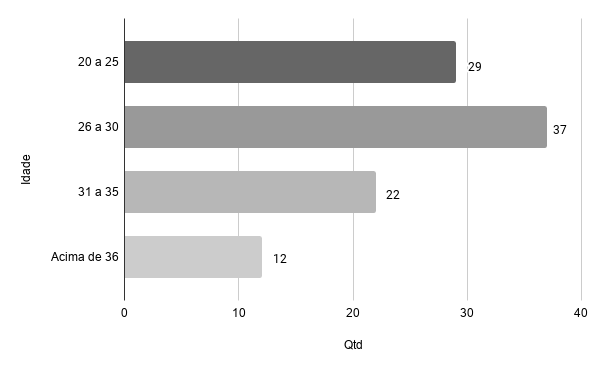
\includegraphics[width=.70\textwidth]{images/s_idade.png}
        \label{figure:s_idade}
        \caption{Idade.}
        \end{figure}
    
    
    %\item Figura \ref{figure:s_escolaridade}: Nível de escolaridade.
        \begin{figure}[!htb]
        \centering
        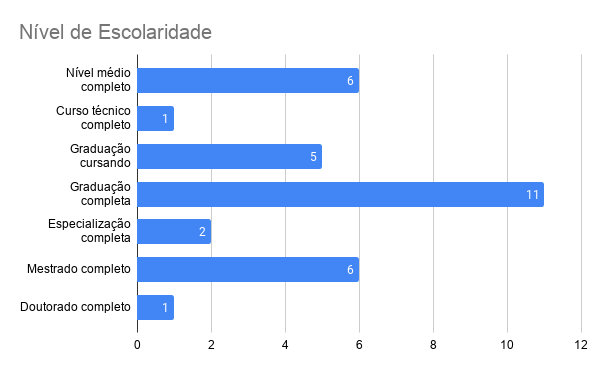
\includegraphics[width=.70\textwidth]{images/s_escolaridade.png}
        \label{figure:s_escolaridade}
        \caption{Nível de escolaridade.}
        \end{figure}
    
    
    %\item Figura \ref{figure:s_areaformacaoacademica}: Área de Formação Acadêmica.
        \begin{figure}[!htb]
        \centering
        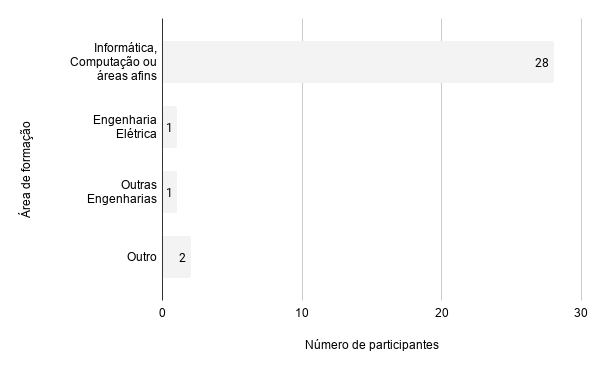
\includegraphics[width=.80\textwidth]{images/s_areaformacaoacademica.png}
        \label{figure:s_areaformacaoacademica}
        \caption{Área de formação acadêmica.}
        \end{figure}
    
    
    %\item Figura \ref{figure:s_certificacao}: Fez algum curso / certificação na área de testes?
        \begin{figure}[!htb]
        \centering
        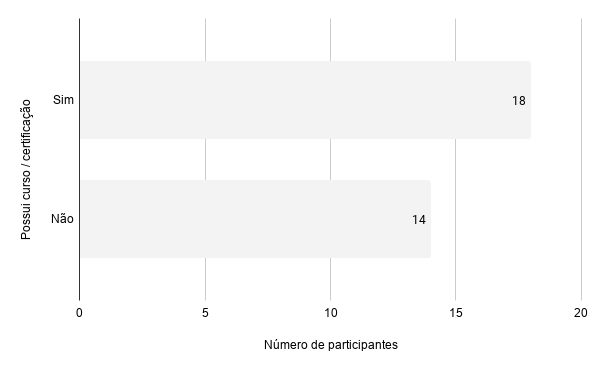
\includegraphics[width=.80\textwidth]{images/s_certificacao.png}
        \label{figure:s_certificacao}
        \caption{Você já fez algum curso / certificação na área de testes?}
        \end{figure}
    
    
    %\item Figura \ref{figure:s_certificacaodesc}: Caso a pergunta acima tenha sido "Sim", quais foram esses cursos / certificações?
        \begin{figure}[!htb]
        \centering
        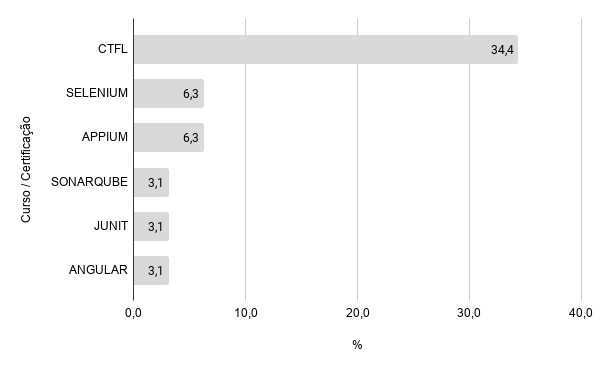
\includegraphics[width=.80\textwidth]{images/s_certificacaodesc.png}
        \label{figure:s_certificacaodesc}
        \caption{Caso a pergunta acima tenha sido "Sim", quais foram esses cursos / certificações?}
        \end{figure}
    
    
    %\item Figura \ref{figure:s_projetos}: Em relação a testes de projetos de apps Android, você:
        \begin{figure}[!htb]
        \centering
        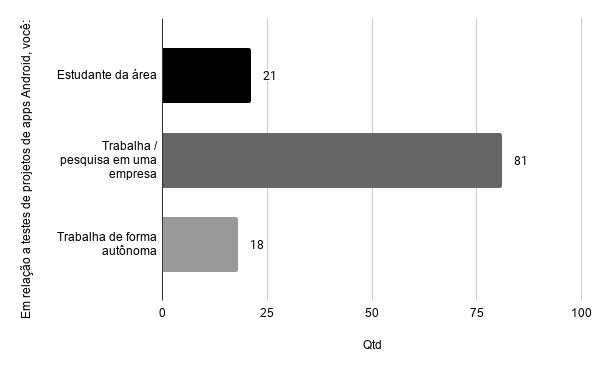
\includegraphics[width=.80\textwidth]{images/s_projetos.png}
        \label{figure:s_projetos}
        \caption{Em relação a testes de projetos de apps Android, você:}
        \end{figure}
    
    
    %\item Figura \ref{figure:s_estado}: Estado onde trabalha / estuda:
        \begin{figure}[!htb]
        \centering
        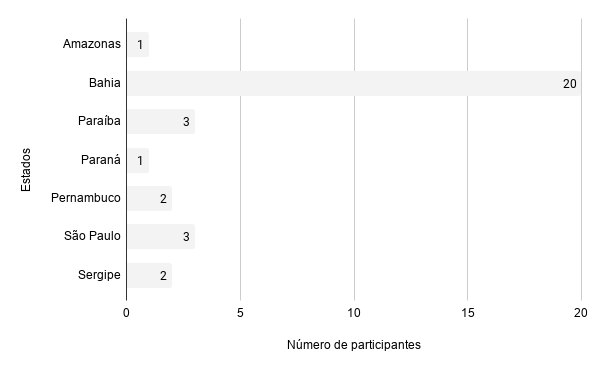
\includegraphics[width=.80\textwidth]{images/s_estado.png}
        \label{figure:s_estado}
        \caption{Estado onde trabalha / estuda:}
        \end{figure}


    %\item Figura \ref{figure:s_experienciatestes}: Experiência profissional na área de TESTES DE SOFTWARE:
        \begin{figure}[!htb]
        \centering
        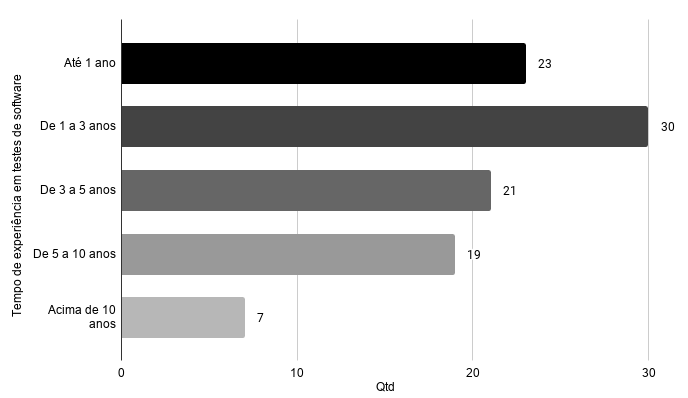
\includegraphics[width=.80\textwidth]{images/s_experienciatestes.png}
        \label{figure:s_experienciatestes}
        \caption{Experiência profissional na área de TESTES DE SOFTWARE:}
        \end{figure}
    

    %\item Figura \ref{figure:s_experienciatestesandroid}: Experiência profissional na área específica de TESTES DE APPS ANDROID:
        \begin{figure}[!htb]
        \centering
        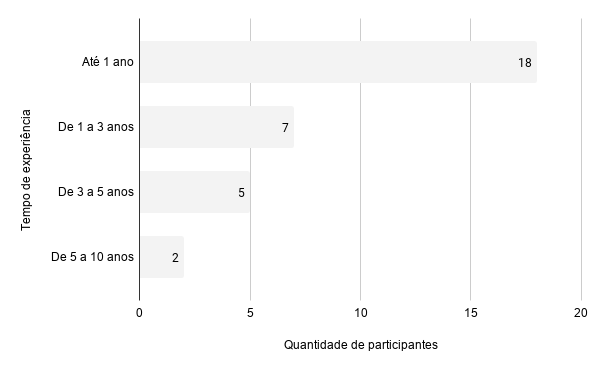
\includegraphics[width=.80\textwidth]{images/s_experienciatestesandroid.png}
        \label{figure:s_experienciatestesandroid}
        \caption{Experiência profissional na área específica de TESTES DE APPS ANDROID:}
        \end{figure}
    
    
     %\item Figura \ref{figure:s_conhecimentotestesandroid}: Quando comparado a outros profissionais, como você considera o seu nível de conhecimento em TESTES DE APPS ANDROID?
        \begin{figure}[!htb]
        \centering
        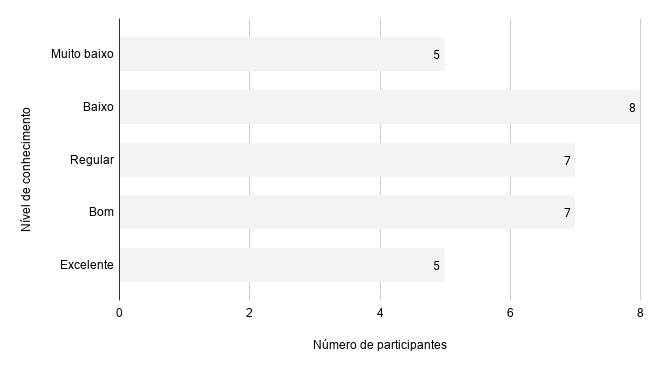
\includegraphics[width=.80\textwidth]{images/s_conhecimentotestesandroid.png}
        \label{figure:s_conhecimentotestesandroid}
        \caption{Quando comparado a outros profissionais, como você considera o seu nível de conhecimento em TESTES DE APPS ANDROID?}
        \end{figure}   
    
    
    \begin{comment}
        %\item Figura \ref{figure:s_funcaoprojeto}: Caso seja funcionário de uma empresa, qual a sua principal função no projeto atual?
        \begin{figure}[!htb]
        \centering
        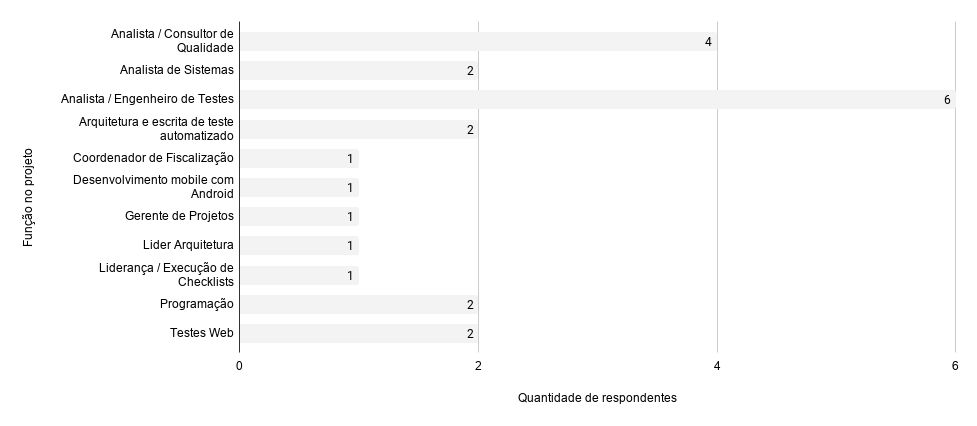
\includegraphics[width=.90\textwidth]{images/s_funcaoprojeto.png}
        \label{figure:s_funcaoprojeto}
        \caption{Caso seja funcionário de uma empresa, qual a sua principal função no projeto atual?}
        \end{figure}
    \end{comment}

    
    
    %\item Figura \ref{figure:s_atividadesprojeto}: Qual(is) atividade(s) realiza no processo de teste de software:
        \begin{figure}[!htb]
        \centering
        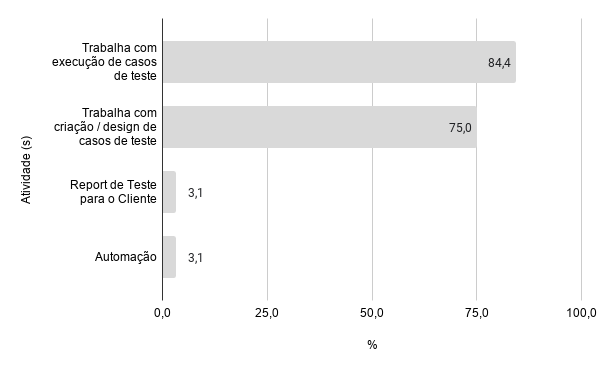
\includegraphics[width=.80\textwidth]{images/s_atividadesprojeto.png}
        \label{figure:s_atividadesprojeto}
        \caption{Qual(is) atividade(s) realiza no processo de teste de software:}
            \end{figure}   
    
    
    %\item Figura \ref{figure:s_categoriastestes}: Os testes realizados se enquadram em qual(is) categorias:
        \begin{figure}[!htb]
        \centering
        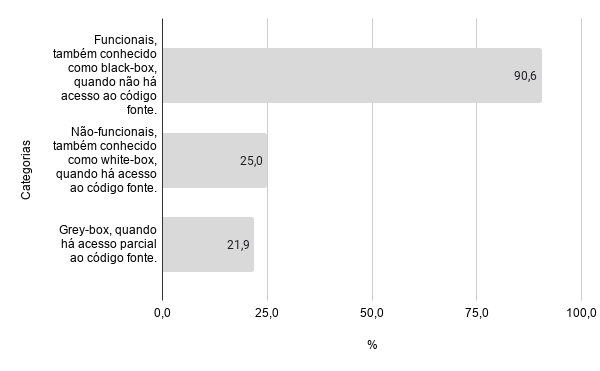
\includegraphics[width=.80\textwidth]{images/s_categoriastestes.png}
        \label{figure:s_categoriastestes}
        \caption{Os testes realizados se enquadram em qual(is) categorias:}
        \end{figure}       
    
  
     %\item Figura \ref{figure:s_tipostestes}: Qual(is) tipo(s) de teste são feitos:
        \begin{figure}[!htb]
        \centering
        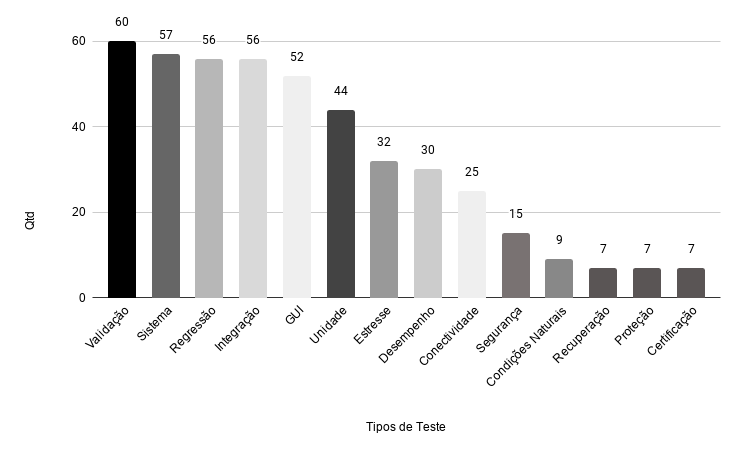
\includegraphics[width=.90\textwidth]{images/s_tipostestes.png}
        \label{figure:s_tipostestes}
        \caption{Qual(is) tipo(s) de teste são feitos:}
        \end{figure}
    
    
     %\item Figura \ref{figure:s_formatestes}: Os testes são realizados de forma:
        \begin{figure}[!htb]
        \centering
        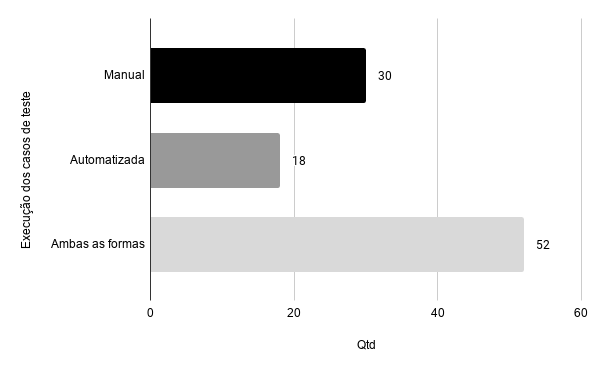
\includegraphics[width=.80\textwidth]{images/s_formatestes.png}
        \label{figure:s_formatestes}
        \caption{Os testes são realizados de forma:}
        \end{figure}    
    
    
    %\item Figura \ref{figure:s_ferramentastestes}: Quais ferramentas você costuma utilizar em seus projetos de APPS ANDROID?
        \begin{figure}[!htb]
        \centering
        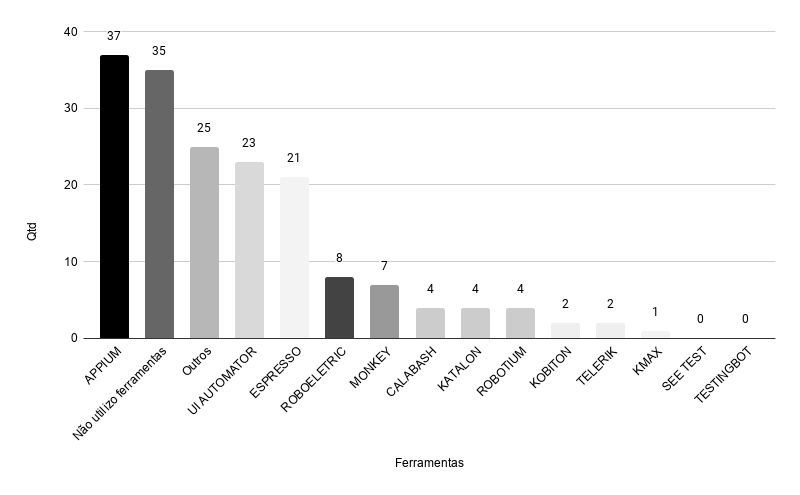
\includegraphics[width=.80\textwidth]{images/s_ferramentastestes.png}
        \label{figure:s_ferramentastestes}
        \caption{Quais ferramentas você costuma utilizar em seus projetos de APPS ANDROID?}
        \end{figure}
    
    
    %\item Figura \ref{figure:s_testemanutencao}: Quando é realizada uma MANUTENÇÃO (ATUALIZAÇÃO) no app Android, quer seja perfectiva, corretiva, adaptativa ou preventiva, é realizado algum tipo de teste com o objetivo de garantir que as manutenções realizadas não alteraram o comportamento funcional do app?
        \begin{figure}[!htb]
        \centering
        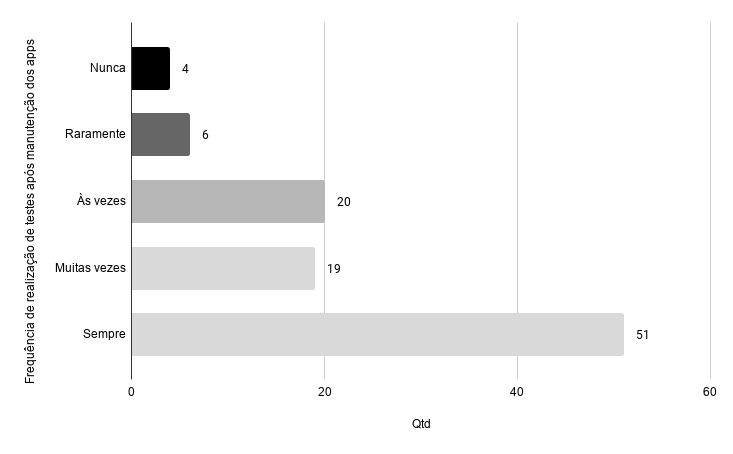
\includegraphics[width=.80\textwidth]{images/s_testemanutencao.png}
        \label{figure:s_testemanutencao}
        \caption{Quando é realizada uma MANUTENÇÃO (ATUALIZAÇÃO) no app Android, quer seja perfectiva, corretiva, adaptativa ou preventiva, é realizado algum tipo de teste com o objetivo de garantir que as manutenções realizadas não alteraram o comportamento funcional do app?}
        \end{figure}   
    
    
    %\item Figura \ref{figure:s_formatestemanutencao}: Caso, a resposta anterior seja positiva, o processo de teste durante MANUTENÇÃO (ATUALIZAÇÃO) do app é feita de que forma?
        \begin{figure}[!htb]
        \centering
        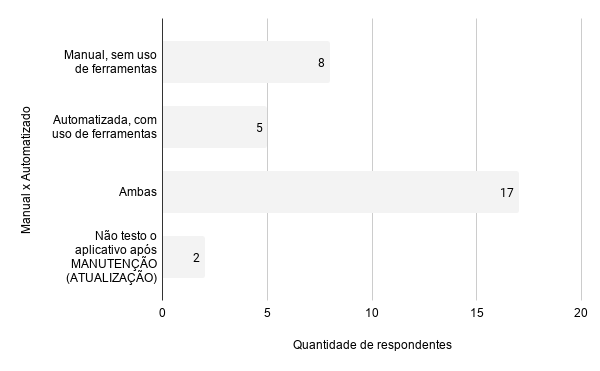
\includegraphics[width=.80\textwidth]{images/s_formatestemanutencao.png}
        \label{figure:s_formatestemanutencao}
        \caption{Caso, a resposta anterior seja positiva, o processo de teste durante MANUTENÇÃO (ATUALIZAÇÃO) do app é feita de que forma?}
        \end{figure}     
    
    
    %\item Figura \ref{figure:s_processostestemanutencao}: Quais processos você realiza para testar a versão atualizada do app:
        \begin{figure}[!htb]
        \centering
        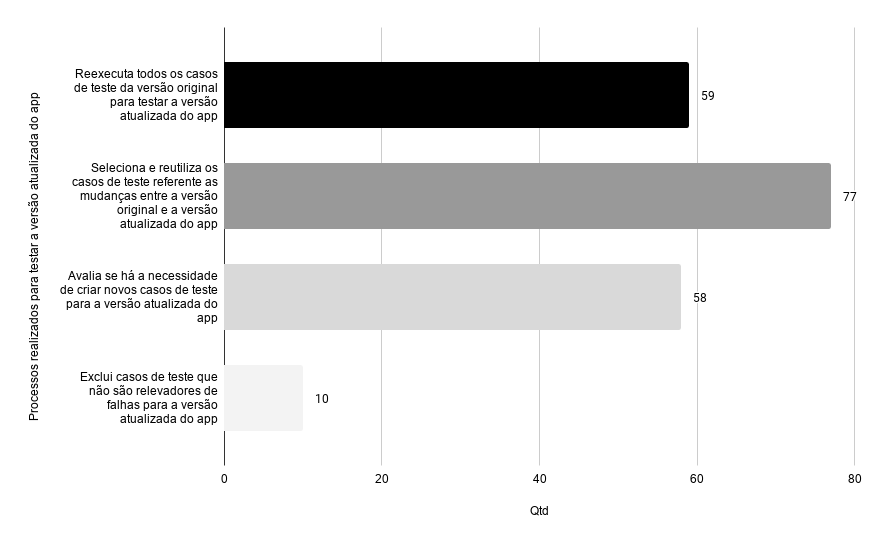
\includegraphics[width=.80\textwidth]{images/s_processostestemanutencao.png}
        \label{figure:s_processostestemanutencao}
        \caption{Quais processos você realiza para testar a versão atualizada do app:}
        \end{figure} 
    
    
    %\item Figura \ref{figure:s_testenovo}: Quando realiza alguma MANUTENÇÃO (ATUALIZAÇÃO) utiliza alguma ferramenta para automatizar o teste da nova versão do APP ANDROID?
        \begin{figure}[!htb]
        \centering
        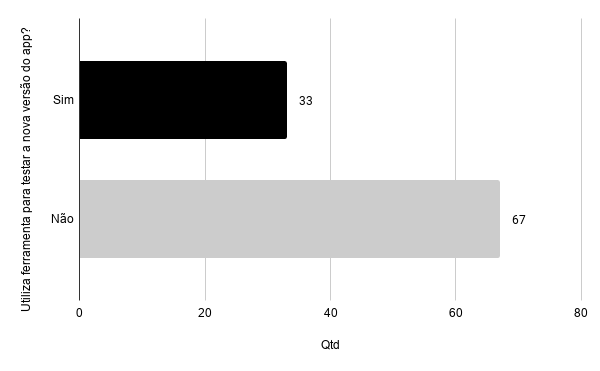
\includegraphics[width=.80\textwidth]{images/s_testenovo.png}
        \label{figure:s_testenovo}
        \caption{Quando realiza alguma MANUTENÇÃO (ATUALIZAÇÃO) utiliza alguma ferramenta para automatizar o teste da nova versão do APP ANDROID?}
        \end{figure}
    
    
    %\item Figura \ref{figure:s_ferramentastestenovo}: Caso utilize, qual(is) são a(s) ferramenta(s)?
        \begin{figure}[!htb]
        \centering
        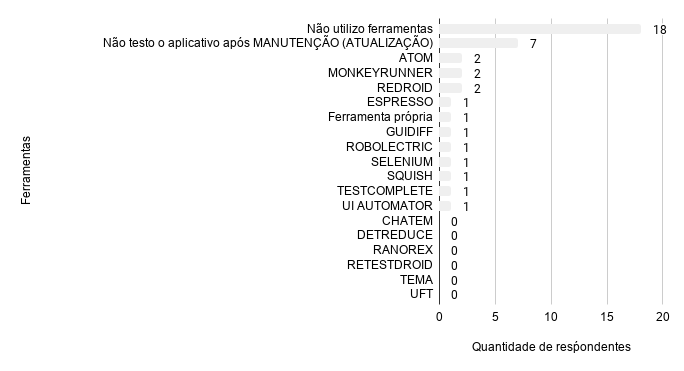
\includegraphics[width=.80\textwidth]{images/s_ferramentastestenovo.png}
        \label{figure:s_ferramentastestenovo}
        \caption{Caso utilize, qual(is) são a(s) ferramenta(s)?}
        \end{figure}
    
    
    %\item Figura \ref{figure:s_ferramentasexpectativas}: A(s) ferramenta(s) utilizada(s) atendem as necessidades para testar o app após ATUALIZAÇÃO (MANUTENÇÃO)?
        \begin{figure}[!htb]
        \centering
        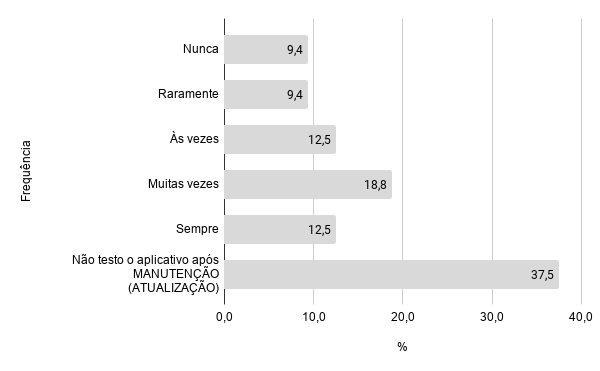
\includegraphics[width=.80\textwidth]{images/s_ferramentasexpectativas.png}
        \label{figure:s_ferramentasexpectativas}
        \caption{A(s) ferramenta(s) utilizada(s) atendem as necessidades para testar o app após ATUALIZAÇÃO (MANUTENÇÃO)?}
        \end{figure}
    
    \begin{comment}
    %\item Figura \ref{figure:s_jferramentasexpectativas}: Justifique a resposta anterior:
        \begin{figure}[!htb]
        \centering
        \includegraphics[width=.80\textwidth]{images/s_jferramentasexpectativas.png}
        \label{figure:s_jferramentasexpectativas}
        \caption{Justifique a resposta anterior:}
        \end{figure}
    \end{comment}
    
    
    %\item Figura \ref{figure:s_imptestarmanutencao}: Considera relevante testar apps ao realizar algum tipo de MANUTENÇÃO (ATUALIZAÇÃO)?
        \begin{figure}[!htb]
        \centering
        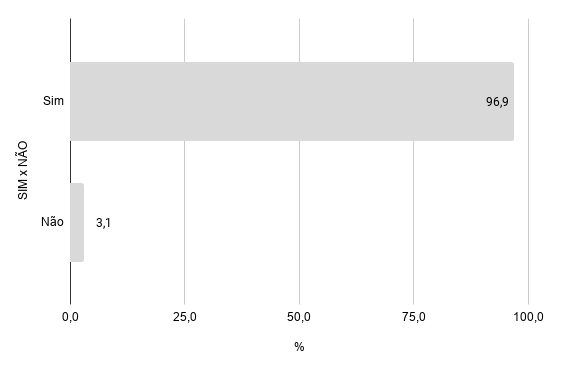
\includegraphics[width=.80\textwidth]{images/s_imptestarmanutencao.png}
        \label{figure:s_imptestarmanutencao}
        \caption{Considera relevante testar apps ao realizar algum tipo de MANUTENÇÃO (ATUALIZAÇÃO)?}
        \end{figure}
    
    
    %\item Figura \ref{figure:s_fatorestestemanutencao}: Qual(is) fator(es) você considera que fazem com que não sejam feitos testes em aplicativos após realização de MANUTENÇÃO (ATUALIZAÇÃO):
        \begin{figure}[!htb]
        \centering
        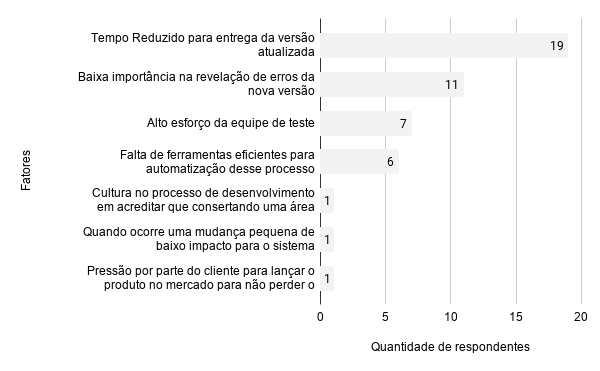
\includegraphics[width=.80\textwidth]{images/s_fatorestestemanutencao.png}
        \label{figure:s_fatorestestemanutencao}
        \caption{Qual(is) fator(es) você considera que fazem com que não sejam feitos testes em aplicativos após realização de MANUTENÇÃO (ATUALIZAÇÃO):}
        \end{figure}
    
   \begin{comment}
     % \item Figura \ref{figure:s_featuresfmanutencao}: Na sua opinião, quais são as features / funcionalidades que as ferramentas de teste precisam implementar para melhorar / automatizar o processo de testes  durante a manutenção de apps Android? Justifique sua resposta.
        \begin{figure}[!htb]
        \centering
        \includegraphics[width=.80\textwidth]{images/featuresfmanutencao.png}
        \label{figure:s_featuresfmanutencao}
   %    \caption{Na sua opinião, quais são as features / funcionalidades que as ferramentas de teste precisam implementar para melhorar / automatizar o processo de testes  durante a manutenção de apps Android? Justifique sua resposta.}
        \end{figure} 
   \end{comment}
   
    
    
    %\item Figura \ref{figure:s_featuresexistentes}: Você está satisfeito(a) com as features  / funcionalidades oferecidas pelas ferramentas de testes de app Android existentes?
        \begin{figure}[!htb]
        \centering
        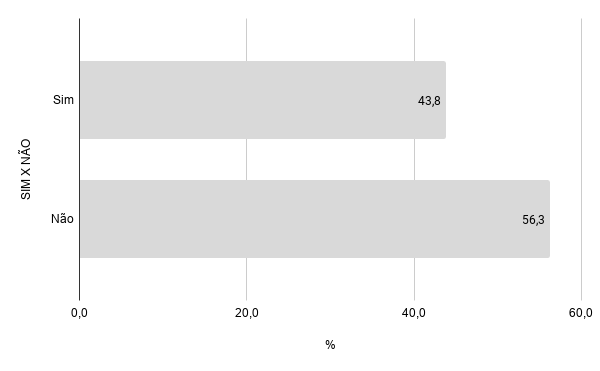
\includegraphics[width=.80\textwidth]{images/s_featuresexistentes.png}
        \label{figure:s_featuresexistentes}
        \caption{Você está satisfeito(a) com as features  / funcionalidades oferecidas pelas ferramentas de testes de app Android existentes?}
        \end{figure}

\begin{comment}
      % \item Figura \ref{figure:s_jfeaturesexistentes}: Justifique a sua resposta:
    \begin{figure}[!htb]
    \centering
    \includegraphics[width=.80\textwidth]{images/s_jfeaturesexistentes.png}
   \label{figure:s_jfeaturesexistentes}
   \caption{Justifique a sua resposta:}
   \end{figure}   
\end{comment}

    
    
%\end{itemize}
















